% Für Bindekorrektur als optionales Argument "BCORfaktormitmaßeinheit", dann
% sieht auch Option "twoside" vernünftig aus
% Näheres zu "scrartcl" bzw. "scrreprt" und "scrbook" siehe KOMA-Skript Doku
\documentclass[12pt,a4paper,titlepage,headinclude]{scrartcl}

%%%%%%%%%%%%%%%%%%%%%%%%%%%%%% Formatierung %%%%%%%%%%%%%%%%%%%%%%%%%%%

%keine Einrückung nach leerzeile
\parindent0pt

% Für Kopf und Fußzeilen, siehe auch KOMA-Skript Doku
\usepackage[komastyle]{scrpage2}
\pagestyle{scrheadings}
\setheadsepline{0.5pt}[\color{black}]
\automark[section]{chapter}

%Zitate und Literaturverzeichnis
\usepackage[backend=bibtex,natbib=true,sorting=nyt,style=numeric-comp]{biblatex}
\usepackage[babel,german=quotes]{csquotes}
\bibliography{literatur}

%Zur vernünftigen Dekodierung
\usepackage[T1]{fontenc} %
\usepackage[utf8]{inputenc} %utfx8
\usepackage[ngerman]{babel} %

%Interaktives Dokument
\usepackage[pdfpagelabels=true]{hyperref}%

%Für wissenschaftliches Zitieren
%\usepackage{natbib}

%Schriftarten
%\usepackage{lmodern} %

%Formatierung für Kof- und Fußzeile. Hier gilt entweder ... oder ...!!

%Für eigenen Zeilenabstand
\usepackage{setspace} %

%Für die Seitenformatierung
\usepackage{lscape} %
\usepackage{multicol} %
\usepackage{wallpaper} %

%Styling Inhaltsverzeichnis
\usepackage{tocloft} %

% Zur Formatierung für Kopf und Fußzeilen. Im Allgemeinen ist scrpage2 besser als fancyhdr
\usepackage{scrpage2}
\pagestyle{scrheadings}
\setheadsepline{0.5pt}[\color{black}]

%Einstellungen für Figuren- und Tabellenbeschriftungen
\setkomafont{captionlabel}{\sffamily\bfseries}
\setcapindent{0em} 


%%%%%%%%%%%%%%%%%%%%%%%%%%%%%% Mathematisches %%%%%%%%%%%%%%%%%%%%%%%%%%%

%Pakete für Mathesymbole
\usepackage{latexsym,exscale,stmaryrd} %
\usepackage{amssymb, amsfonts, amstext} %
\usepackage{amsmath, mathtools, amsthm} %

%align nummerierung
\numberwithin{equation}{subsection}

% Weitere Symbole
\usepackage[nointegrals]{wasysym} %
\usepackage{eurosym} %
\usepackage{textcomp} %

%\usepackage{ucs} %

%Für vernünftige Einheiten 
\usepackage[separate-uncertainty, exponent-product = \cdot]{siunitx}
%\usepackage[thinspace,thinqspace,amssymb]{SIunits} %
\usepackage{icomma} %
\usepackage{nicefrac}%

%SI-Einheiten
\usepackage{siunitx}

%%%%%%%%%%%%%%%%%%%%%%%%%%%%%% Grafiken & Tabellen %%%%%%%%%%%%%%%%%%%%%%%%%%%
% Text umfließt Graphiken und Tabellen
% Beispiel:
% \begin{wrapfigure}[Zeilenanzahl]{"l" oder "r"}{breite}
%   \centering
%   \includegraphics[width=...]{grafik}
%   \caption{Beschriftung} 
%   \label{fig:grafik}
% \end{wrapfigure}
% Mehrere Abbildungen nebeneinander
% Beispiel:
% \begin{figure}[htb]
%   \centering
%   \subfigure[Beschriftung 1\label{fig:label1}]
%   {\includegraphics[width=0.49\textwidth]{grafik1}}
%   \hfill
%   \subfigure[Beschriftung 2\label{fig:label2}]
%   {\includegraphics[width=0.49\textwidth]{grafik2}}
%   \caption{Beschriftung allgemein}
%   \label{fig:label-gesamt}
% \end{figure}

%Subfigure nur mit PDF statt Bildern einfügen:
\usepackage{adjustbox}
%\begin{figure}[h]
%  \centering
%  \subfigure[Caption1\label{fig:bild1}]
%  {\begin{adjustbox}{width=0.44\linewidth}\input{bild1}\end{adjustbox}}
%  \hfill
%  \subfigure[Caption2\label{bild2}]
%  {\begin{adjustbox}{width=0.44\linewidth}\input{bild2}\end{adjustbox}}
%  \hfill
%  \subfigure[Caption3\label{bild3}]
%  {\begin{adjustbox}{width=0.44\linewidth}\input{bild3}\end{adjustbox}}
%  \caption{Gesamtcaption}
%  \label{fig:gesamtlabel}
%\end{figure}

%\usepackage{subfigure}




% Caption neben Abbildung
% Beispiel:
% \sidecaptionvpos{figure}{"c" oder "t" oder "b"}
% \begin{SCfigure}[rel. Breite (normalerweise = 1)][hbt]
%   \centering
%   \includegraphics[width=0.5\textwidth]{grafik.png}
%   \caption{Beschreibung}
%   \label{fig:}
% \end{SCfigure}

%Einstellungen für Figuren- und Tabellenbeschriftungen
\setkomafont{captionlabel}{\sffamily\bfseries}
\setcapindent{0em}

%Fuer mehr Platz in den Tabellen
\usepackage{cellspace} %mehr Platz in Tabellen
\addtolength\cellspacetoplimit{3pt}
\newcommand\myhline[1][2pt]{\\[#1]\hline}

%Zum Einbinden von GRafiken
\usepackage{graphicx}% [pdflatex]
\usepackage{xcolor}%

%Für textumflossene Grafiken
\usepackage{wrapfig} %

%Für subfigure
\usepackage{caption}
\usepackage{subcaption}

% Caption neben Abbildung
\usepackage{sidecap}

%Für URLs
\usepackage{url}%

%Zum Einbinden von Quelltext
\usepackage{listings-ext} %

%Für chemische Formeln
\usepackage{chemfig} %
%Für chemische Formeln (von www.dante.de)
%% Anpassung an LaTeX(2e) von Bernd Raichle
\makeatletter
\DeclareRobustCommand{\chemical}[1]{%
  {\(\m@th
   \edef\resetfontdimens{\noexpand\)%
       \fontdimen16\textfont2=\the\fontdimen16\textfont2
       \fontdimen17\textfont2=\the\fontdimen17\textfont2\relax}%
   \fontdimen16\textfont2=2.7pt \fontdimen17\textfont2=2.7pt
   \mathrm{#1}%
   \resetfontdimens}}
\makeatother
%erzwinge Fussnote auf selber Seite
\interfootnotelinepenalty=1000

%Zusätzliche Boxen
\usepackage{fancybox}

%\usepackage{framed}
%\usepackage{mathmode}
%\usepackage{empheq}

%Für variable Referenzen
\usepackage{varioref}

%Für Tabellen mit fester Gesamtbreite und variabler Spaltenbreite (im Gegensatz zu tabular)
\usepackage{tabularx}
%\newcommand{\ltab}{\raggedright\arraybackslash} % Tabellenabschnitt linksbündig
%\newcommand{\ctab}{\centering\arraybackslash} % Tabellenabschnitt zentriert
%\newcommand{\rtab}{\raggedleft\arraybackslash} % Tabellenabschnitt rechtsbündig


%Für Gleitobjekte
\usepackage{float} %Für H-Option

\usepackage{multirow} % Zellen von Tabellen zusammenfassen
\usepackage{booktabs} % verschoenert Tabellen
\usepackage{fixltx2e} % Repariert einige Dinge in Bezug auf das setzen von Gleitobjekten http://ctan.org/pkg/fixltx2e
\usepackage{stfloats} % Bei Gleitobjekten (figure,table,...) die ueber zwei Spalten gesetzt werden (Umgebung figure*), funktioniert [tb] http://ctan.org/pkg/stfloats
\usepackage{rotating} % Wird für Text und Grafiken benötigt, die um einen Winkel gedreht werden sollen



%%%%%%%%%%%%%%%%%%%%%%%%%%%%%% Kommandodefinitionen %%%%%%%%%%%%%%%%%%%%%%%%%%%

%Zur Korrektur und Kommentierung
\newcommand{\comment}[1]{\marginpar{\tiny{\textcolor{red}{#1}}}} % ermoeglicht kleine Kommentare am Seitenrand: \comment{Fehler?}
\newcommand{\Comment}[1]{\textcolor{red}{#1}}

%Zur Formatierung in der Matheumgebung
\renewcommand{\t}{\ensuremath{\rm\tiny}} % Tiefgestellter Text in der Matheumgebung wird schoener mit: $\Phi_{\t{Text}}$
\renewcommand{\d}{\ensuremath{\mathrm{d}}} % Die totale Ableitung ist stets aufrecht zu setzen: \d
\newcommand{\diff}[3][]{\ensuremath{\frac{\d^{#1}#2}{\d#3^{#1}}}} % einfache Ableitung nach x: $\ddx{\Phi}$
\newcommand{\pdiff}[3][]{\ensuremath{\frac{\partial^{#1}#2}{\partial#3^{#1}}}} % wie gesprochen, eine partielle Ableitung: \del
\newcommand{\aeqiv}{\ensuremath{\qquad \Longleftrightarrow \qquad}} % Eine Aequivalenz
\newcommand{\folgt}{\ensuremath{\qquad \Longrightarrow \qquad}} % Ein Folgepfeil mit Abstaenden
\newcommand{\corresponds}{\ensuremath{\mathrel{\widehat{=}}}} % Befehl für "Entspricht"-Zeichen
\newcommand{\mi}[1]{\ensuremath{\mathit{#1}}} % italics für griechische Buchstaben in Matheumgebung

%Um nicht so viel schreiben zu müssen...
\newcommand{\bs}[1]{\boldsymbol{#1}}
\newcommand{\ol}[1]{\overline{#1}}
\newcommand{\wtilde}[1]{\widetilde{#1}}
\newcommand{\mrm}[1]{\mathrm{#1}}
\newcommand{\mbf}[1]{\mathbf{#1}}
\newcommand{\mbb}[1]{\mathbb{#1}}
\newcommand{\mcal}[1]{\mathcal{#1}}
\newcommand{\mfrak}[1]{\mathfrak{#1}}

%Abkürzungen
\newcommand{\zB}{z.\,B.\ }
\newcommand{\bzw}{b.\,z.\, w.\ }
\newcommand{\Dh}{d.\,h.\ }
\newcommand{\Gl}{Gl.\ }
\newcommand{\Abb}{Abb.\ }
\newcommand{\Tab}{Tab.\ }

%Farbige Box um eine Formel
%Anwendung:
%\eqbox{
%  \begin{equation}
%    ...
%  \end{equation}
%}
\newcommand{\eqbox}[1]{
  \colorbox{gray!30}{\parbox{\linewidth}{#1}} 
}

%Im Text
\newcommand{\engl}[1]{engl. \textit{#1}}
\newcommand{\zitat}[1]{\footnote{#1}}
\newcommand{\person}[1]{\textsc{#1}}


%Matheoperatoren
\DeclareMathOperator{\tr}{tr}
\DeclareMathOperator{\sgn}{sgn}
\DeclareMathOperator{\diag}{diag}
\DeclareMathOperator{\const}{const}
\DeclareMathOperator{\grad}{grad}
\DeclareMathOperator{\rot}{rot}
\DeclareMathOperator{\divz}{div}


%%%%%%%%%%%%%%%%%%%%%%%%% Quellcode - Formatierung %%%%%%%%%%%%%%%%%%%%%%%%%%%%%%%%%%%%%%

%Um auch Umlaute in den Kommentaren auswerten zu können
\lstset{
literate = {Ö}{{\"O}}1 {Ä}{{\"A}}1 {Ü}{{\"U}}1 {ß}{{\ss}}2 {ü}{{\"u}}1
           {ä}{{\"a}}1 {ö}{{\"o}}1
}

%Formatierung des Quellcode
\lstset{
language=C++,
basicstyle=\footnotesize\ttfamily,
keywordstyle=\bfseries\color{blue},
stringstyle=\color{red},
commentstyle=\itshape\color{green!60!black},
emphstyle = \bfseries\color{red!80!green!60!blue}
%identifierstyle=,
}

%Zum Hervorheben bestimmter Begriffe (z.B. eigene Klassen, etc.)
%\lstset{
%emph = {vector, iterator, std, ostream, istream , ofstream, ifstream, fstream, cmath}
%}

%Nummerirung
\lstset{
numbers=left,
numberstyle=\tiny,
stepnumber=2,
numbersep=5pt,
frame=single,
breaklines=true
framesep=5pt,
numbersep=8pt,
breakindent=3ex
}

%Einbunden über
%\lstinputlisting[caption={blablabla}, language=C++]{name.cpp}

\begin{document}
%Autor, etc.
\newcommand{\titel}{Wetter, Druck und Höhe \& Tornado}
\newcommand{\praktikant}{Kevin Lüdemann}
\newcommand{\email}{
      \href{mailto:kevin.luedemann@stud.uni-goettingen.de}
           {kevin.luedemann@stud.uni-goettingen.de} }
\newcommand{\durchfuehrungsdatum}{07.12.2015}
\newcommand{\abgabedatum}{02.01.2016}

%Metainformationen
\hypersetup{
      pdfauthor = {\praktikant~ },
      pdftitle  = {\titel},
      pdfsubject = {\titel}
}

\begin{titlepage}
\centering
\textsc{\Large Experiementelle Verfahren der Strömungsmechanik,\\[1.5ex] DLR Göttingen}

\vspace*{2.5cm}

\rule{\textwidth}{1pt}\\[0.5cm]
{\huge \bfseries
  \titel}\\[0.5cm]
\rule{\textwidth}{1pt}

\vspace*{2.5cm}

\begin{Large}
\begin{tabular}{ll}
Praktikanten: &  \praktikant,\\
Email:	& \email\\
Durchgeführt am: & \durchfuehrungsdatum\\
Abgegeben am: & \abgabedatum\\
\end{tabular}
\end{Large}
\vspace*{0.8cm}
\end{titlepage}
\pagenumbering{arabic}

\newpage

\section{Wetter}
\subsection{Momentane Lage}
In der Stunde der Durchführung waren am Himmel so gut, wie nur Stratos Wolken zu sehen.
An einigen Wolkenlöchern konnte man aber auch ein paar Altocumulus Wolken erkennen.
Die deutet auf eine durchgehend homogene Bewölkung aufgrund von Zwischenzohnenwetter hin.
Dies wird weiter von dem nur leichten Wind bestätigt.
Dieser lies sich aber aufgrund seiner nur sehr geringen Stärke keine ausgeprägten Richtung zuordnen.
Dies sind ähnliche Bedingungen, wie im Rücklagenwetter, allerdings zeigt sich dieses auch durch eine geringe Bewölkung.
Ebenfalls regnete es zum Zeitpunkt der Messung nicht, aber im Laufe des Nachmittags gab es einie Regentropfen.
Die Temperatur war eher Mild und rund um 13$\si{\celsius}$.
Diese schwankten aber auch nicht start im laufe des Nachmittags.\\
Hierraus lässt sich ableiten, dass sich das Wetter auch in den weiteren Stunden nicht stark ändern wird.
Ohne Wind können sich die Wolken nicht weiter bewegen und somit bleibt auch die Temperatur annähernd konstant, wenn es keinen spontanen Regenschauer mehr giebt.


\subsection{Wetter aus Druckkarten}
\begin{figure}[!h]
\centering
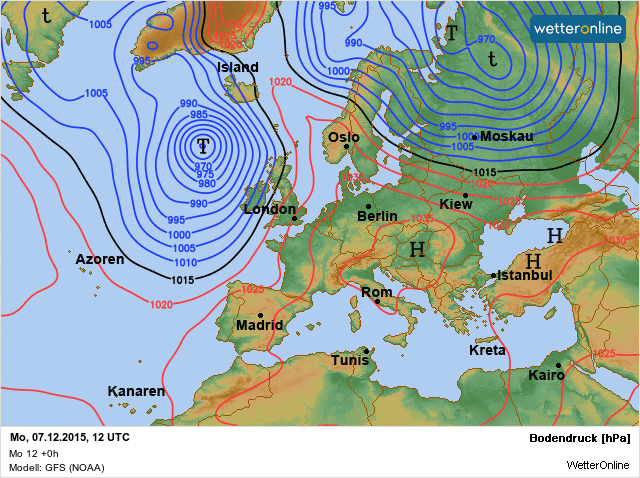
\includegraphics[width=0.7\textwidth]{wetter0712.png}
\caption{Druckkarte Europas für den 07.12.2015 entnommen aus wetteronline.de}
\label{fig:w0712}
\end{figure}
Die Druckkarte vom Tag der Praktikumsdurchführung dem 07.12.2015 ist in der Abbildung \ref{fig:w0712} zu sehen.
Aus dieser Druckkarte kann man entnemen, dass über Rusland und Nordeuropa, sowie über dem Atlantik südlich von Island sich jeweils ein starkausgeprägtes Tiefdruckgebiet befindet.
Dem gegebüber liegt über Zentraleuropa ein stark ausgeprägtes Hochdruckgebiet.
Dieses Hoch bestimmt das Wetter in ganz Deutschland.
Speziell für die Region Göttingen ist ein kleiner Druckgradient zu erkennen, welcher an den weit auseinander liegenden Isobaren zu sehen ist.
Dies bedeutet, das es eher keinen bzw. leichten Wind gibt.
Diese kommt aufgrund der rechtsdrehung des Hochdruckgebietes aus Süd-Westen, somit ist die Windrichtung Nord-Ost.

\begin{figure}[!h]
\centering
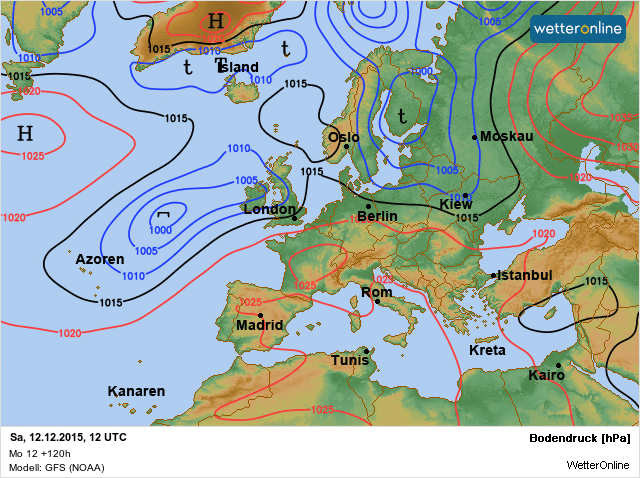
\includegraphics[width=0.7\textwidth]{wetter1212.png}
\caption{Druckkarte Europas für den 12.12.2015 entnommen aus wetteronline.de}
\label{fig:w1212}
\end{figure}
Die Druckvorhersage für den 12.12.2015 ist in der Abbildung \ref{fig:w1212} zu sehen.
Hier ist zu erkennen, dass sich das Hochduckgebiet in Richtung Süd-Süd-Ost bewegt.
Desweiteren bewegen sich die Tiefdruckgebiete aufeinander zu und scheinen sich zu einem Gebiet zu vereinigen.
Ebenfalls ist zu erkennen, dass das neu verbundene Tiefdruckgebiet deutlich schwächer ist im gegensatz zum Hochdruckebiet, dass immernoch gut ausgeprägt ist.
Diese Bewegung sorgt für eine Wetteränderung in der Region Göttingen, da nun langsam der Druck sinkt und sich die Ausläufer des Tiefs bemerkbar machen.
Dies sorgt für zunehmenden Wind, der vermehrt aus Westen kommt.

\begin{figure}[!h]
\centering
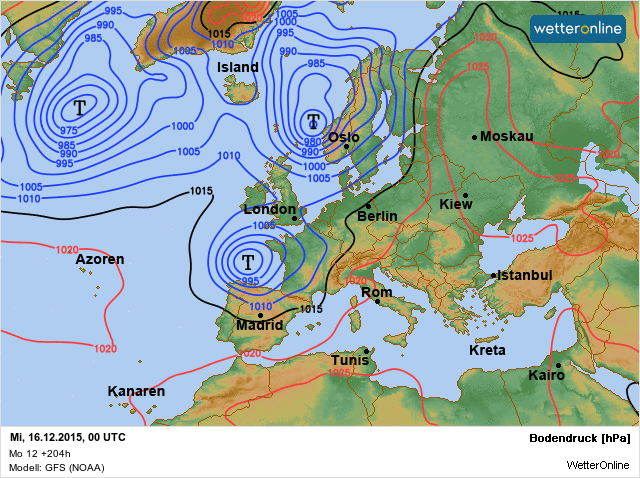
\includegraphics[width=0.7\textwidth]{wetter1612.png}
\caption{Druckkarte Europas für den 16.12.2015 entnommen aus wetteronline.de}
\label{fig:w1612}
\end{figure}
Die Druckvorhersage für den 16.12.2015 ist in der Abbildung \ref{fig:w1612} zu sehen.
Hier ist zu erkennen, dass die Tiefdruckgebiete nun in Richtung Mitteleuropa wandern und auch an stäke zulegen.
Zu dem zieht ein weiteres Tiefdruckgebiet von Nord-Westen nach Europa.
Das Hochdruckgebiet, dass sich noch über Mitteleuropa befand wandert weiter Richtung Nord-Ost und somit nach Russland.
Die Tiefdruckgebiete über dem Raum Göttingen werden für stärkeren Wind und vermehrt für Regen sorgen.
Speziell für den Raum Göttingen bleibt die eher milde Westwindströmung erhalten.
Dies sorgt weiterhin für milde Temperaturen und fehlenden Schnee.

\begin{figure}[!h]
\centering
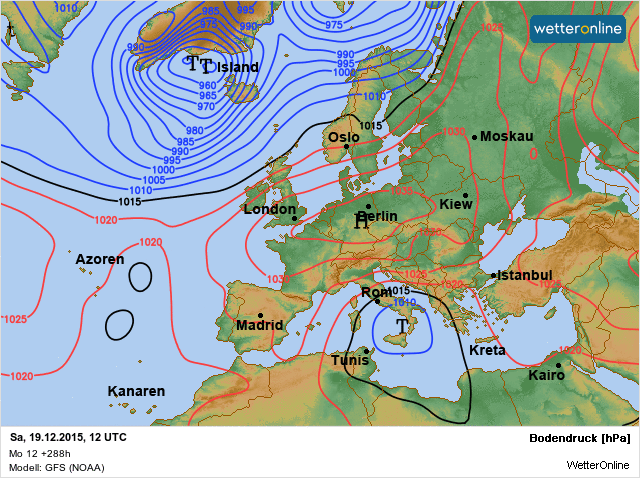
\includegraphics[width=0.7\textwidth]{wetter1912.png}
\caption{Druckkarte Europas für den 19.12.2015 entnommen aus wetteronline.de}
\label{fig:w1912}
\end{figure}
Für den 19.12.2015 ist die Druckvorhersage in der Abbildung \ref{fig:w1912} zu sehen.
Hier zeigt sich jetzt, dass sich eines der Tiefdruckgebiete gelöst hat und weiter richtung Süd-Osten gewandert ist.
Es wird durch einen Hochdruckrücken von den anderen Tiefdruckgebieten über Skandinavien getrennt.
Dieser Hochdruckrücken erstreckt sich von Süd-Westen bis Nord-Osten über Mitteleuropa und sorgt auch hier weiterhin für milde Luft aus dem Mittelmeer Raum.
Allerdings nimmt der Wind wieder ab und es bahnen sich keine starken Wetterveränderungen in den nächsten Tagen an.
Dies liegt auch daran, dass die Tiefdruckgebiete an stärke verloren haben.

\begin{figure}[!h]
\centering
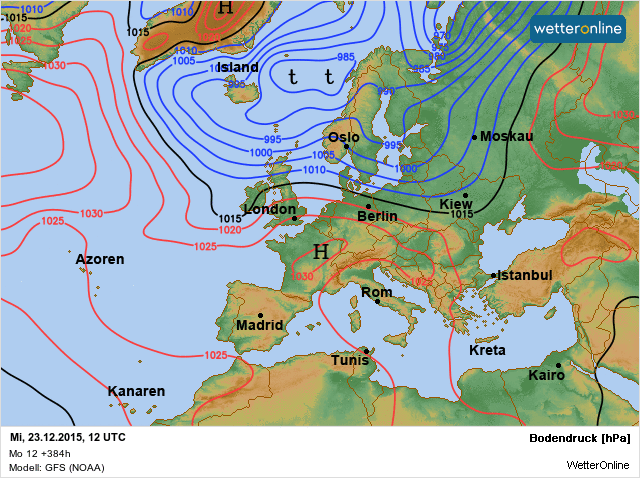
\includegraphics[width=0.7\textwidth]{wetter2312.png}
\caption{Druckkarte Europas für den 23.12.2015 entnommen aus wetteronline.de}
\label{fig:w2312}
\end{figure}
Die letzte Druckvorhersage für den 23.12.2015 ist in der Abbildung \ref{fig:w2312} zu sehen.
Über Mitteleuropa herscht weiterhin der Einfluss eines Hochdruckgebietes, welches sich nun aber weiter gegen Nord-Westen ausgedeht hat und nun auch Luft aus Richtung Grönland zu uns transportiert.
Dies kann sorgt für etwas kältere Temperaturen.
Allerdings sind die Tiefdruckgebiete über Skandinavien immer noch eher schwach und somit ist auch der Wind nicht sonderlich stark.
Somit hällt sich die milde Lust noch ein weile über Mitteleuropa und die Temperaturen ändern sich auch nur leicht.
Die Aussicht auf weiße Weihnachten ist eher gering, da nicht viel kalten Polarluft in Richtung Norddeutschland geschaufelt wird.

\section{Druck und Höhe}
\label{sec:durchfuehrung}
\subsection{Theoretische Grundlagen}
Die Höhe hängt logarithmisch von der Höhe ab.
Dies ergibt sich aus der Eulergleichung\cite[114]{gerthsen}
\begin{align*}
	\frac{\partial\vec{v}}{\partial t}+\left( \vec{v}\cdot\nabla\right)\vec{v}=-\frac{1}{\rho} \nabla p+ \vec{g}
\end{align*}
für den statischen und stationären Fall.
Sprich das Geschwindigkeitsfeld ist konstant.
Hierbei ist $\vec{g}$ die Erdbeschleunigung, welche in Richtung $-z$ zeigt und nur mit $g$ bezeichnet wird.
Somit vereinfacht sich die Gleichung zu 
\begin{align*}
	\nabla p =& -\rho\vec{g}\\
	\Rightarrow \frac{\partial p}{\partial z} =& -\rho g
\end{align*}
und somit zu einer reinen Höhenabhägigkeit in die $z$ Richtung.
Ersetzt man die Dichte aus der Idealgasgleichung\cite[260]{gerthsen} mit $\rho=\frac{pM}{RT}$, wobei $M$ die Masse, $T$ die Temperatur und $R$ die Gaskonstante ist, bekommt man eine Abhängigkeit von der sogenanten Druckscalenhöhe $h_s=\frac{RT}{Mg}$.
Diese Gleichung lässt sich jetzt durch integration Lösen und ergibt die Barometrische Höhenformel
\begin{align}
	\Delta h(h) = h_s\ln{\frac{p(h_0)}{p(h)}}\label{eq:hoehe},
\end{align}
wobei $\Delta h$ die Höhendifferen von $h_0$ und $h$ ist. 

\subsection{Durchführung}
Um die Abhängigkeit von der Höhe und dem Druck zu messen, wird ein Druckmessgerät mit einer maximalen Auflösung von $\sigma_p=1\si{\pascal}$ verwendet.
Es wird das Gebäute des DLR\_School\_lab von der untersten Ebene bis zur höchsten in einzelnen Schritten vermessen.
Um die Fehler gering zu halten muss die Druckmessung möglichst schnell erfolgen, da wie man anhand der Gleichung \eqref{eq:hoehe} erkennen kann der Druck von der Temperatur abhängt und diese in Gebäuden um mehrer grad Kelvin schwanken kann.
Dennoch müssen Schwankungen in der Elektrik ausgeglichen werden, in dem über eine gewissen Zeitraum gemittel wird.
Dieser betrug bei der Messung etwa $30\si{\second}$.\\
Im Anschluss an die Messung des Drucks wird mithilfe eines Maßbandes die Höhendifferenz der einzelnen Etagen mit einer Genauigkeit von $\sigma_h=3\si{\centi\meter}$ vermessen, welche durch das Maßband und die unzugänglichkeit der Etagen zu begründen ist.

\subsection{Ergebnisse}
\begin{figure}[!h]
\centering
% GNUPLOT: LaTeX picture with Postscript
\begingroup
  \makeatletter
  \providecommand\color[2][]{%
    \GenericError{(gnuplot) \space\space\space\@spaces}{%
      Package color not loaded in conjunction with
      terminal option `colourtext'%
    }{See the gnuplot documentation for explanation.%
    }{Either use 'blacktext' in gnuplot or load the package
      color.sty in LaTeX.}%
    \renewcommand\color[2][]{}%
  }%
  \providecommand\includegraphics[2][]{%
    \GenericError{(gnuplot) \space\space\space\@spaces}{%
      Package graphicx or graphics not loaded%
    }{See the gnuplot documentation for explanation.%
    }{The gnuplot epslatex terminal needs graphicx.sty or graphics.sty.}%
    \renewcommand\includegraphics[2][]{}%
  }%
  \providecommand\rotatebox[2]{#2}%
  \@ifundefined{ifGPcolor}{%
    \newif\ifGPcolor
    \GPcolorfalse
  }{}%
  \@ifundefined{ifGPblacktext}{%
    \newif\ifGPblacktext
    \GPblacktexttrue
  }{}%
  % define a \g@addto@macro without @ in the name:
  \let\gplgaddtomacro\g@addto@macro
  % define empty templates for all commands taking text:
  \gdef\gplbacktext{}%
  \gdef\gplfronttext{}%
  \makeatother
  \ifGPblacktext
    % no textcolor at all
    \def\colorrgb#1{}%
    \def\colorgray#1{}%
  \else
    % gray or color?
    \ifGPcolor
      \def\colorrgb#1{\color[rgb]{#1}}%
      \def\colorgray#1{\color[gray]{#1}}%
      \expandafter\def\csname LTw\endcsname{\color{white}}%
      \expandafter\def\csname LTb\endcsname{\color{black}}%
      \expandafter\def\csname LTa\endcsname{\color{black}}%
      \expandafter\def\csname LT0\endcsname{\color[rgb]{1,0,0}}%
      \expandafter\def\csname LT1\endcsname{\color[rgb]{0,1,0}}%
      \expandafter\def\csname LT2\endcsname{\color[rgb]{0,0,1}}%
      \expandafter\def\csname LT3\endcsname{\color[rgb]{1,0,1}}%
      \expandafter\def\csname LT4\endcsname{\color[rgb]{0,1,1}}%
      \expandafter\def\csname LT5\endcsname{\color[rgb]{1,1,0}}%
      \expandafter\def\csname LT6\endcsname{\color[rgb]{0,0,0}}%
      \expandafter\def\csname LT7\endcsname{\color[rgb]{1,0.3,0}}%
      \expandafter\def\csname LT8\endcsname{\color[rgb]{0.5,0.5,0.5}}%
    \else
      % gray
      \def\colorrgb#1{\color{black}}%
      \def\colorgray#1{\color[gray]{#1}}%
      \expandafter\def\csname LTw\endcsname{\color{white}}%
      \expandafter\def\csname LTb\endcsname{\color{black}}%
      \expandafter\def\csname LTa\endcsname{\color{black}}%
      \expandafter\def\csname LT0\endcsname{\color{black}}%
      \expandafter\def\csname LT1\endcsname{\color{black}}%
      \expandafter\def\csname LT2\endcsname{\color{black}}%
      \expandafter\def\csname LT3\endcsname{\color{black}}%
      \expandafter\def\csname LT4\endcsname{\color{black}}%
      \expandafter\def\csname LT5\endcsname{\color{black}}%
      \expandafter\def\csname LT6\endcsname{\color{black}}%
      \expandafter\def\csname LT7\endcsname{\color{black}}%
      \expandafter\def\csname LT8\endcsname{\color{black}}%
    \fi
  \fi
    \setlength{\unitlength}{0.0500bp}%
    \ifx\gptboxheight\undefined%
      \newlength{\gptboxheight}%
      \newlength{\gptboxwidth}%
      \newsavebox{\gptboxtext}%
    \fi%
    \setlength{\fboxrule}{0.5pt}%
    \setlength{\fboxsep}{1pt}%
\begin{picture}(7200.00,5040.00)%
    \gplgaddtomacro\gplbacktext{%
      \csname LTb\endcsname%
      \put(946,704){\makebox(0,0)[r]{\strut{}$-2$}}%
      \put(946,1518){\makebox(0,0)[r]{\strut{}$-1.5$}}%
      \put(946,2332){\makebox(0,0)[r]{\strut{}$-1$}}%
      \put(946,3147){\makebox(0,0)[r]{\strut{}$-0.5$}}%
      \put(946,3961){\makebox(0,0)[r]{\strut{}$0$}}%
      \put(946,4775){\makebox(0,0)[r]{\strut{}$0.5$}}%
      \put(1078,484){\makebox(0,0){\strut{}$-2$}}%
      \put(1714,484){\makebox(0,0){\strut{}$0$}}%
      \put(2350,484){\makebox(0,0){\strut{}$2$}}%
      \put(2986,484){\makebox(0,0){\strut{}$4$}}%
      \put(3622,484){\makebox(0,0){\strut{}$6$}}%
      \put(4259,484){\makebox(0,0){\strut{}$8$}}%
      \put(4895,484){\makebox(0,0){\strut{}$10$}}%
      \put(5531,484){\makebox(0,0){\strut{}$12$}}%
      \put(6167,484){\makebox(0,0){\strut{}$14$}}%
      \put(6803,484){\makebox(0,0){\strut{}$16$}}%
    }%
    \gplgaddtomacro\gplfronttext{%
      \csname LTb\endcsname%
      \put(176,2739){\rotatebox{-270}{\makebox(0,0){\strut{}Relativdruck $\Delta p$ [hPa]}}}%
      \put(3940,154){\makebox(0,0){\strut{}Höhe $h$ [m]}}%
      \csname LTb\endcsname%
      \put(5816,4602){\makebox(0,0)[r]{\strut{}Messwerte}}%
      \csname LTb\endcsname%
      \put(5816,4382){\makebox(0,0)[r]{\strut{}Lin. Reg.}}%
    }%
    \gplbacktext
    \put(0,0){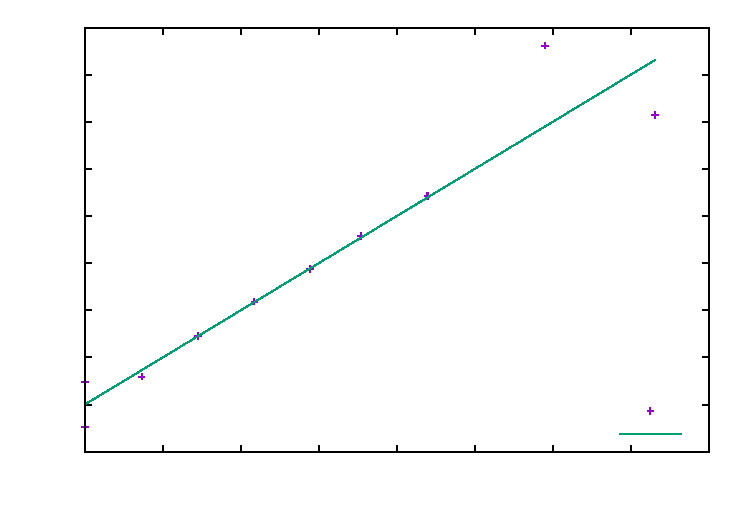
\includegraphics{hoehe}}%
    \gplfronttext
  \end{picture}%
\endgroup

\caption{Zusammenhang zwischen gemessener Höhe und aus dem Druck berechneter Höhe. Zur Veranschaulichung wurde eine Ursprungsgerade mit Steigung 1 gezeichnet.}
\label{fig:hoehe}
\end{figure}
Die gemessenen Daten sind in der Abbildung \ref{fig:hoehe} zu sehen.
In dieser Abbildung ist die Höhe mithilfe der Gleichung \eqref{eq:hoehe} aus den gemessenen Druckdaten umgerechnet worden.
Hierbei ist der Logarithmus aufgrund der kleinen Höhenänderung linear approximiert worden.
Die gemessenen Höhendaten sind als x-Achse aufgetragen.
Mithilfe der eingezeichneten Ursprungsgeraden mit Steigung 1, lässst sich das Gesetz der Barometrischen Höhenformel und der linearisierung für die im Gebäude erreichten Höhen gut darstellen.
Es ist zu erkennen, dass die Höhe gerade für die ersten $10\si{\meter}$ mit der Theorie übereinstimmt.\\
Ab dieser Höhe aber weichen die Werte stark von den zu erwartenden Werten ab.
Die ist unter anderem mit der höheren Ungenauigkeit der Messung mithilfe des Maßbandes zu erklären.
Für die letzten zwei Messpunkte war das genau ablesen nicht mehr einfach Möglich, aufgrund der Geometrie des Gebäudes.
Zu dem war das Maßband aufgrund seines Eigengewichtes nicht mehr in einer stabilen Position zu halten.
Diese beiden Fehlerquellen erhöhen den Messfehler auf mindestens $\sigma_h=1\si{\deci\meter}$.
Desweiteren, war das Gebäude beheitzt, was zu Änderungen der Temperatur führte, je höher man sich im Gebäude befindet.
Dennoch ist für die meisten Messwerte das Gesetz nachgewiesen worden.\\
Um die Messung zu optimieren, müssen die freien Parameter eliminiert werden.
Dieser ist im Fall der Druckmessung die Temperatur.
Diese muss für die gesamte Messung konstant gehalten werden, sprich auch für die gesamte Höhe.
Da warme Luft aufsteigt, darf das Gebäude nicht beheitzt werden, bzw. muss, wenn es beheitzt wird eine homogene Temperatur anehmen.
Letzteres ist aber nur schwer umzusetzten.
Die praktikable Lösung ist hier das Gebäude in thermisches Gleichgewicht mit der umgebenen Luft zu bringen, so hat jede Höhenmessung auch die gleiche Temperatur, da die Außentemperatur als konstant für die Dauer der Messung angenommen werden kann.

\section{Tornadoexperiment}
\subsection{Theorie}
Tornados sind in der Theorie noch nicht im Deteil verstanden.
Es gibt aber zur Beschreibung einiger Parameter ein einfaches Modell.\\
Für die Geschwindigkeit $v$ innerhalb und außerhalb des Tornados gibt es das Modell des Rankin Wirbels\footnote{https://de.wikipedia.org/wiki/Wirbel\_(Strömungslehre)}.
Der Tornado wird somit als ein Wirbel beschrieben.
Ebenfalls nimmt das Model an, dass der Wirbel einen Druchmesser $R$ hat.
Für die Geschwindigkeit ergibt sich somit
\begin{align}
	v(r) = 
	\begin{cases}
		\omega r & \text{falls } r \leq R\\ 
		\omega \frac{R^2}{r} & \text{falls } r > R\label{eq:rw}\\
	\end{cases}
\end{align}
eine Abhängigkeit im Wirbel, die mit $r$ dem Radius linear wächst und außerhalb des Wirbels, wie $\frac{1}{r}$ abfällt.
Hierbeit ist $\omega$ die Winkelgeschwindigkeit des Wirbelkerns.


\subsection{Durchführung}
Im Experiment wird ein vom DLR bereitgestellter Tornadosimulator verwendet.
Dieser bietet die Möglichkeit das Geschwindigkeitsfeld des Wirbels an verschiedenen Stellen über den Betrag der Geschwindigkeit zu bestimmen.
Dazu wird eine Messonde in den Wirbel eingebracht und diese kann den Betrag der Geschwindigkeit messen.
Der Tornado befindet sich in einem geschlossenen Messaufbau und kann deswegen als Zylindersymmetrisch angenommen werden.
Dadurch braucht die Geschwindigkeitsänderung nur radial nach außen gemessen zu werden.
Dies wird für veschiedene Höhen wiederholt.

\subsection{Ergebnisse}

\begin{figure}[!h]
\centering
% GNUPLOT: LaTeX picture with Postscript
\begingroup
  \makeatletter
  \providecommand\color[2][]{%
    \GenericError{(gnuplot) \space\space\space\@spaces}{%
      Package color not loaded in conjunction with
      terminal option `colourtext'%
    }{See the gnuplot documentation for explanation.%
    }{Either use 'blacktext' in gnuplot or load the package
      color.sty in LaTeX.}%
    \renewcommand\color[2][]{}%
  }%
  \providecommand\includegraphics[2][]{%
    \GenericError{(gnuplot) \space\space\space\@spaces}{%
      Package graphicx or graphics not loaded%
    }{See the gnuplot documentation for explanation.%
    }{The gnuplot epslatex terminal needs graphicx.sty or graphics.sty.}%
    \renewcommand\includegraphics[2][]{}%
  }%
  \providecommand\rotatebox[2]{#2}%
  \@ifundefined{ifGPcolor}{%
    \newif\ifGPcolor
    \GPcolortrue
  }{}%
  \@ifundefined{ifGPblacktext}{%
    \newif\ifGPblacktext
    \GPblacktexttrue
  }{}%
  % define a \g@addto@macro without @ in the name:
  \let\gplgaddtomacro\g@addto@macro
  % define empty templates for all commands taking text:
  \gdef\gplbacktext{}%
  \gdef\gplfronttext{}%
  \makeatother
  \ifGPblacktext
    % no textcolor at all
    \def\colorrgb#1{}%
    \def\colorgray#1{}%
  \else
    % gray or color?
    \ifGPcolor
      \def\colorrgb#1{\color[rgb]{#1}}%
      \def\colorgray#1{\color[gray]{#1}}%
      \expandafter\def\csname LTw\endcsname{\color{white}}%
      \expandafter\def\csname LTb\endcsname{\color{black}}%
      \expandafter\def\csname LTa\endcsname{\color{black}}%
      \expandafter\def\csname LT0\endcsname{\color[rgb]{1,0,0}}%
      \expandafter\def\csname LT1\endcsname{\color[rgb]{0,1,0}}%
      \expandafter\def\csname LT2\endcsname{\color[rgb]{0,0,1}}%
      \expandafter\def\csname LT3\endcsname{\color[rgb]{1,0,1}}%
      \expandafter\def\csname LT4\endcsname{\color[rgb]{0,1,1}}%
      \expandafter\def\csname LT5\endcsname{\color[rgb]{1,1,0}}%
      \expandafter\def\csname LT6\endcsname{\color[rgb]{0,0,0}}%
      \expandafter\def\csname LT7\endcsname{\color[rgb]{1,0.3,0}}%
      \expandafter\def\csname LT8\endcsname{\color[rgb]{0.5,0.5,0.5}}%
    \else
      % gray
      \def\colorrgb#1{\color{black}}%
      \def\colorgray#1{\color[gray]{#1}}%
      \expandafter\def\csname LTw\endcsname{\color{white}}%
      \expandafter\def\csname LTb\endcsname{\color{black}}%
      \expandafter\def\csname LTa\endcsname{\color{black}}%
      \expandafter\def\csname LT0\endcsname{\color{black}}%
      \expandafter\def\csname LT1\endcsname{\color{black}}%
      \expandafter\def\csname LT2\endcsname{\color{black}}%
      \expandafter\def\csname LT3\endcsname{\color{black}}%
      \expandafter\def\csname LT4\endcsname{\color{black}}%
      \expandafter\def\csname LT5\endcsname{\color{black}}%
      \expandafter\def\csname LT6\endcsname{\color{black}}%
      \expandafter\def\csname LT7\endcsname{\color{black}}%
      \expandafter\def\csname LT8\endcsname{\color{black}}%
    \fi
  \fi
  \setlength{\unitlength}{0.0500bp}%
  \begin{picture}(7200.00,5040.00)%
    \gplgaddtomacro\gplbacktext{%
      \csname LTb\endcsname%
      \put(814,704){\makebox(0,0)[r]{\strut{} 2}}%
      \put(814,1156){\makebox(0,0)[r]{\strut{} 3}}%
      \put(814,1609){\makebox(0,0)[r]{\strut{} 4}}%
      \put(814,2061){\makebox(0,0)[r]{\strut{} 5}}%
      \put(814,2513){\makebox(0,0)[r]{\strut{} 6}}%
      \put(814,2966){\makebox(0,0)[r]{\strut{} 7}}%
      \put(814,3418){\makebox(0,0)[r]{\strut{} 8}}%
      \put(814,3870){\makebox(0,0)[r]{\strut{} 9}}%
      \put(814,4323){\makebox(0,0)[r]{\strut{} 10}}%
      \put(814,4775){\makebox(0,0)[r]{\strut{} 11}}%
      \put(946,484){\makebox(0,0){\strut{} 0}}%
      \put(1597,484){\makebox(0,0){\strut{} 2}}%
      \put(2248,484){\makebox(0,0){\strut{} 4}}%
      \put(2898,484){\makebox(0,0){\strut{} 6}}%
      \put(3549,484){\makebox(0,0){\strut{} 8}}%
      \put(4200,484){\makebox(0,0){\strut{} 10}}%
      \put(4851,484){\makebox(0,0){\strut{} 12}}%
      \put(5501,484){\makebox(0,0){\strut{} 14}}%
      \put(6152,484){\makebox(0,0){\strut{} 16}}%
      \put(6803,484){\makebox(0,0){\strut{} 18}}%
      \put(176,2739){\rotatebox{-270}{\makebox(0,0){\strut{}$v$ [$\frac{\text{m}}{\text{s}}$]}}}%
      \put(3874,154){\makebox(0,0){\strut{}$r$ [cm]}}%
    }%
    \gplgaddtomacro\gplfronttext{%
      \csname LTb\endcsname%
      \put(5816,4602){\makebox(0,0)[r]{\strut{}$20,$cm hoch}}%
      \csname LTb\endcsname%
      \put(5816,4382){\makebox(0,0)[r]{\strut{}$30,$cm hoch}}%
      \csname LTb\endcsname%
      \put(5816,4162){\makebox(0,0)[r]{\strut{}f1(x)}}%
      \csname LTb\endcsname%
      \put(5816,3942){\makebox(0,0)[r]{\strut{}f2(x)}}%
      \csname LTb\endcsname%
      \put(5816,3722){\makebox(0,0)[r]{\strut{}g1(x)}}%
      \csname LTb\endcsname%
      \put(5816,3502){\makebox(0,0)[r]{\strut{}g2(x)}}%
    }%
    \gplbacktext
    \put(0,0){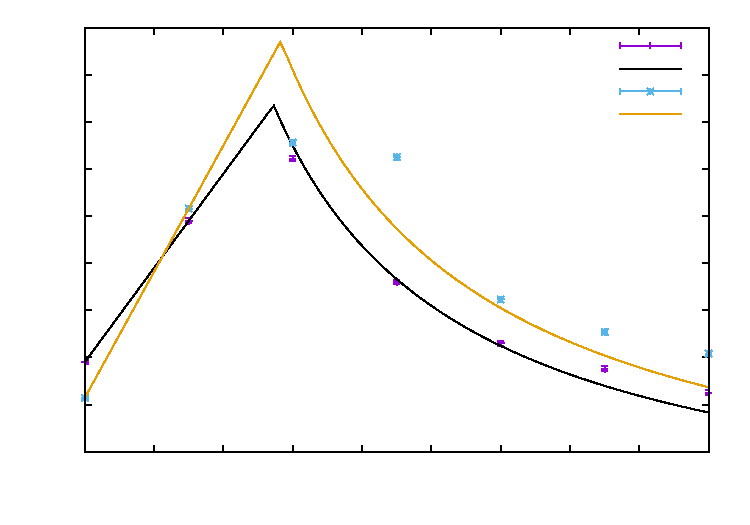
\includegraphics{tornado}}%
    \gplfronttext
  \end{picture}%
\endgroup

\caption{Ergebnisse der Messung des Betrags der Geschwindigkeit im Tornadosimulator. Es wurde die Geschwindigkeit gegen die Tiefe des Wirbels aufgetragen. Die Kurven bilden das jeweils angepasste Rankin Wirbel Modell nach Gleichung \eqref{eq:rw}.}
\label{fig:torn1}
\end{figure}
Die Anwendung des Rankin Wirbel Modells ist in der Abbildung \ref{fig:torn1} zu sehen.
Hierbei sind die Messwerte der Geschwindigkeit für die zwei verschiedenen Höhen gegen die jeweilige Tiefe im Wirbel aufgetragen.
Da bei der Messung der Wirbelkern nich genau zu erkennen war, wurde ebenfalls angenommen, dass die Messreihe den Kern nicht zwangsweise erreicht hat.
Die Kurven, die in der Abbildung zu erkennen sind, stellen das jeweilige Modell der Gleichung \eqref{eq:rw} dar.
Hierbei, war auch der Radius des Tornados einer der Parameter.\\
Wie man erkennen kann stellt das Modell den Betrag der Geschwindigkeit in radialer Richtung bei einer Höhe von $20\si{\centi\meter}$ gut dar.\\
Bei der Kurve für eine Höhe von $30\si{\centi\meter}$ liegen einige der Werte außerhalb des Wirbels nicht mehr auf der vorausgesagten Kurve.
Dies lässt sich darauf zurückführen, dass bei dieser Messung zum einen die Geschwindigkeit nicht ganz radial nach außen gemessen werden konnte.
Dabei war die Hauptfehlerquelle die Annahme, dass der Wirbel ortsfest und Zylindersymmetrisch ist.
Im Experiment zeigte sich, dass der Wirbel, die ganze Zeit in Bewegung war und somit nicht genau gemessen werden konnte.
Dieser Fehler tritt stärker auf, je höher sich die Sonde befindet, da aufgrund der Bauweise des Simulators in Bodennähe die größte Stabilität härschte.



%\newpage
\printbibliography[heading=bibintoc]
\end{document}
